% Which model size for which task (total parameters, logarithmic scale).
% ---------------------------------------------------------------------------
% style.tex --- shared preamble for every figure in book/figures/tikz/
%
% One style for all figures: Latin Modern, thin black lines, a light grey
% fill, and one accent colour used only to mark what is untrusted or wrong.
% Build with scripts/build_figures.sh; see book/figures/README.md.
% ---------------------------------------------------------------------------
\documentclass[tikz,border=6pt]{standalone}
\usepackage[T1]{fontenc}
\usepackage{lmodern}
\usetikzlibrary{arrows.meta,positioning,shapes.geometric,calc,fit,backgrounds}

\hyphenpenalty=10000   % short lines in boxes: ragged, never hyphenated

\definecolor{lightgrey}{gray}{0.92}
\definecolor{accent}{HTML}{9B2D20}

\tikzset{
  every picture/.style={
    line width=0.6pt,
    font=\small,
    >={Stealth[length=5pt,width=4pt]},
    node distance=14pt and 24pt,
  },
  % shapes
  box/.style={draw, rectangle, inner xsep=8pt, inner ysep=5pt,
              minimum height=22pt, align=center},
  grey/.style={box, fill=lightgrey},
  rounded/.style={box, rounded corners=9pt},
  decision/.style={draw, diamond, aspect=2.4, inner sep=1.5pt, align=center},
  group/.style={draw, dashed, rounded corners=5pt, inner sep=7pt},
  % text
  tag/.style={font=\footnotesize, align=center, inner sep=2pt},
  note/.style={font=\footnotesize\itshape, align=center, inner sep=2pt},
  code/.style={font=\small\ttfamily},
  codetag/.style={font=\footnotesize\ttfamily, align=center, inner sep=2pt},
  title/.style={font=\small\scshape, align=center, inner sep=2pt},
  % lines
  arrow/.style={->},
  back/.style={->, dashed},
  thin/.style={line width=0.4pt, gray},
  % the one accent, for what is untrusted, wrong or missing
  bad/.style={accent},
  badbox/.style={box, draw=accent, text=accent},
}

\begin{document}
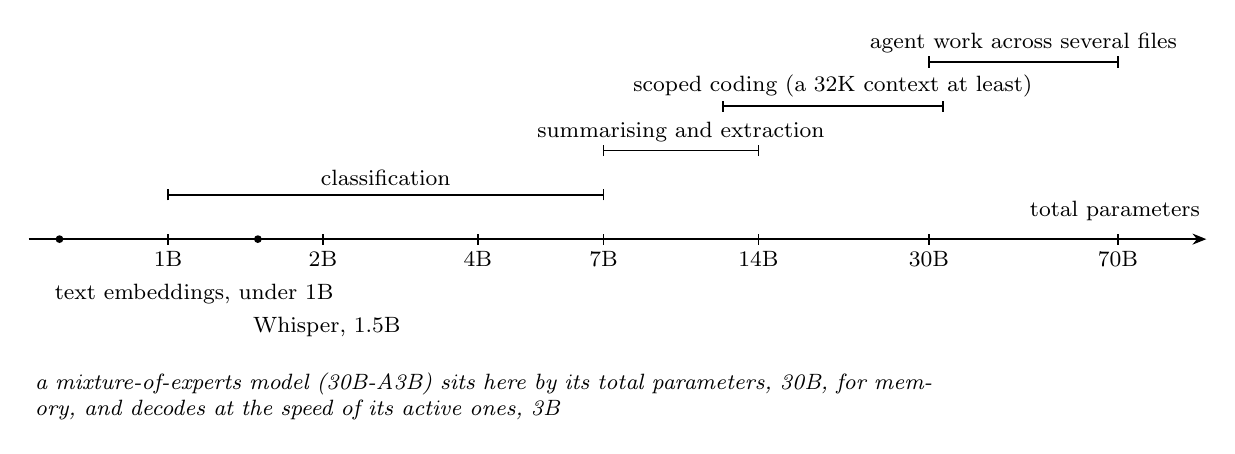
\begin{tikzpicture}[x=56pt]
  % axis: position = log2(parameters in billions)
  \draw[->] (-0.9,0) -- (6.7,0);
  \foreach \p/\l in {0/1B,1/2B,2/4B,2.81/7B,3.81/14B,4.91/30B,6.13/70B}
    \draw (\p,-2pt) -- (\p,2pt) node[tag, below=4pt] {\l};
  \node[tag, anchor=east] at (6.7,10pt) {total parameters};
  % brackets
  \foreach \a/\b/\y/\l in {
      0/2.81/16/classification,
      2.81/3.81/32/summarising and extraction,
      3.58/5.0/48/scoped coding (a 32K context at least),
      4.91/6.13/64/agent work across several files}
    { \draw (\a,\y pt) -- (\b,\y pt);
      \draw (\a,\y pt-2pt) -- (\a,\y pt+2pt);
      \draw (\b,\y pt-2pt) -- (\b,\y pt+2pt);
      \node[tag, above=1pt] at ({(\a+\b)/2},\y pt) {\l}; }
  % marks below
  \fill (-0.7,0) circle (1.4pt) node[tag, below=14pt, anchor=north west, xshift=-4pt] {text embeddings, under 1B};
  \fill (0.58,0) circle (1.4pt) node[tag, below=26pt, anchor=north west, xshift=-4pt] {Whisper, 1.5B};
  \node[note, anchor=north west, text width=330pt, align=left] at (-0.9,-46pt)
    {a mixture-of-experts model (30B-A3B) sits here by its total parameters, 30B, for memory, and decodes at the speed of its active ones, 3B};
\end{tikzpicture}
\end{document}
